\documentclass[11pt,a4paper]{article}
\usepackage[margin=0.95in]{geometry}
\usepackage{amsmath,amssymb}
\usepackage{booktabs}
\usepackage{graphicx}
\usepackage{cite}
\usepackage{tikz}
\usetikzlibrary{positioning,arrows.meta}
\usepackage{setspace}
\setstretch{1.225}
\setlength{\parskip}{0.35em}
\setlength{\parindent}{1.15em}

\title{YOLO and Image Tracking\\[0.4em]
\large How a one-stage detector follows objects from frame to frame}
\author{Computer Science\\ System Design and Optimization}
\date{}

\begin{document}
\maketitle
\thispagestyle{empty}
\vspace{-1.6em}
\noindent\textbf{Keywords---}object detection, YOLO, instance segmentation, multi-object tracking, Kalman filter, data association.

\begin{abstract}
\noindent
YOLO is a family of one-stage object detectors. A single network looks at an image once and returns boxes, class scores, and, in the segmentation variants, a mask for each object. Image tracking is the next question: which box in this frame is the same physical object as a box in the previous frame. This note explains both steps in the setting of a gate camera that sees the side of a stack of beer crates. The detector is the YOLO-vf-seg baseline of the thesis. The tracker is not part of that thesis. The counting system specified there books one sharp frame and does not keep an identity across the buffer, because a union of cells over the passage made the count worse. The pages below separate those two jobs. Detection says what is in this image. Tracking says which of those things have been seen before.
\end{abstract}

\section{What the detector is asked to return}

A still image does not contain a count and it does not contain an identity. It contains intensities. A detector is a function from those intensities to a list. Each entry of the list is a rectangle, a class, and a confidence. A segmenter adds a mask: the set of pixels that belong to that rectangle's object rather than to its neighbor. A tracker adds nothing to a single image. It adds a link between lists that were produced at different times.

The crate passage makes the list concrete. The camera stands at the side of a warehouse gate and sees the front face of returnable beer crates on a forklift. A face is nominally $0.40\,\mathrm{m}$ wide and $0.28\,\mathrm{m}$ high, and the crate is $0.30\,\mathrm{m}$ deep. Six body colors are in use. The useful outputs of one frame are therefore a mask per visible front crate, a center that can be snapped to a lattice, and a color. The useful output of several frames, if a tracker is running, is a stable name for each crate while the forklift moves through the field of view. Those are different products. Mixing them is how a passage gets counted twice.

Two-stage detectors, of which Faster R-CNN is the reference, first propose regions and then classify each region~\cite{ren2015faster}. The second stage is accurate and it is a second look. YOLO's original claim was that a grid of predictors, trained together, can emit the list in one evaluation~\cite{redmon2016yolo}. The claim is about computation and about training, not about magic. The network still has a deep backbone. ``One look'' means one forward pass and a shared set of features, not a shallow glance.

The rest of this note follows one frame through that forward pass, then follows the same object into the next frame. Section~\ref{sec:grid} fixes the box and the score. Section~\ref{sec:net} describes the backbone, neck, and head. Section~\ref{sec:line} records what changed between the 2016 model and the segmenter on the crate line. Section~\ref{sec:nms} treats overlap. Section~\ref{sec:mask} treats the mask. Section~\ref{sec:track} defines a track. Sections~\ref{sec:kalman} and~\ref{sec:assign} derive the prediction and the assignment. Section~\ref{sec:modern} places appearance and low-score boxes. Section~\ref{sec:passage} computes how far a crate moves between two frames of the specified gate. Section~\ref{sec:count} says what that motion must not be used to count.

\section{The grid, the box, and the score}
\label{sec:grid}

The first YOLO divided the image into an $S\times S$ grid. A cell was responsible for an object whose center fell inside it. Each cell predicted $B$ boxes and one set of class probabilities. A box carried a center relative to the cell, a width and a height relative to the image, and a confidence. The confidence was defined as
\begin{equation}
c = \Pr(\mathrm{object})\cdot \mathrm{IoU}(\mathrm{box},\mathrm{truth}),
\label{eq:conf}
\end{equation}
and the class scores were multiplied by $c$ at test time~\cite{redmon2016yolo}. The product is a ranking key. It is not a calibrated probability that the crate is amber, and it is not a licence to add the scores and call the sum a count.

The intersection over union of two boxes $A$ and $B$ is
\begin{equation}
\mathrm{IoU}(A,B) = \frac{|A\cap B|}{|A\cup B|}.
\label{eq:iou}
\end{equation}
If the boxes are axis-aligned, both areas are products of width and height. For two boxes of equal size $w\times h$ whose centers differ by $d$ along the width and not at all along the height, and for $d<w$,
\begin{equation}
\mathrm{IoU} = \frac{w-d}{w+d}.
\label{eq:iou-shift}
\end{equation}
Equation~\eqref{eq:iou-shift} is the only overlap formula this note needs. It says that a detector which has moved its box by a quarter of the object's width still overlaps the old box at $(0.75)/(1.25)=0.60$, and that a move by most of the width drives the overlap near zero. Tracking will reuse that fact.

The one-class-per-cell rule was the sharp limit of the first model. Two crate centers that fell in one cell could not both be typed. Later versions removed the limit by predicting class scores per box, or per anchor, and by using several feature scales so that a small crate and a large crate are not forced through the same cell size~\cite{redmon2018yolov3}. The grid remains a useful picture. Modern heads are dense: many spatial locations each emit a small set of box parameters. A location is still ``responsible'' in the loose sense that its receptive field and its training assignment cover the objects whose centers land nearby.

A box may be parameterized in more than one way. The early models predicted a center and a size directly, then switched to offsets from anchor boxes whose shapes were clustered on the training set~\cite{redmon2017yolo9000}. Anchor-free heads, which YOLOX brought into this family and which YOLOv8 keeps, predict the distances from a point on the object to the four sides of the box~\cite{ge2021yolox}. The four distances determine the rectangle. No catalog of prior shapes has to match a $0.40\times 0.28$ face photographed at $2.5\,\mathrm{m}$. That is a practical advantage on a gate where the scale is set by the camera mount rather than by the variety of anchor clusters in a public dataset.

Objectness, in the versions that still emit it, is a separate score for ``there is an object here,'' trained against the boxes that the assignment procedure marked positive. YOLOv3 used a logistic objectness and independent logistic classifiers, so two labels could both be active~\cite{redmon2018yolov3}. A crate line does not need multi-label boxes. A face is one color. The score that matters operationally is the one that will survive non-maximum suppression and then be handed to a color head or to a tracker. A low score is not the same event as a missing crate. ByteTrack, discussed later, is built on that distinction~\cite{zhang2022bytetrack}.

\section{Backbone, neck, and head}
\label{sec:net}

The forward pass splits into three duties. The backbone turns the image into a stack of feature maps at decreasing resolution. The neck mixes those maps so that a high-resolution map can carry semantics from a deep map. The head reads the mixed maps and emits boxes, classes, and, when asked, mask coefficients.

ResNet showed that a very deep stack can be trained if layers learn residuals~\cite{he2016resnet}. Darknet-53, the YOLOv3 backbone, is a residual stack of $3\times 3$ and $1\times 1$ convolutions with a similar motive~\cite{redmon2018yolov3}. CSPNet then split the feature map so that part of the gradient skips a block of convolutions instead of being recomputed through it~\cite{wang2020cspnet}. That split is the ancestor of the cross-stage modules in the later YOLO backbones, including the one YOLOv8 uses. None of this structure knows what a crate is. It is a way to spend depth on a $1280$-pixel-wide frame without the memory of a detector that runs a second network on every proposal.

The neck is a feature pyramid~\cite{lin2017fpn}. A top-down path carries coarse semantics down to fine maps, and lateral connections add the detail that the coarse map had thrown away. A bottom-up path, as in PANet, then carries the restored detail back up, so the large-object head is not starved of edges~\cite{liu2018panet}. YOLOv4 and its successors use that bidirectional idea~\cite{bochkovskiy2020yolov4}. On the crate face the objects are nearly the same size, so the pyramid is not earning its keep by detecting both a forklift and a bottle cap. It earns its keep at the lips. A lip is a thin horizontal edge. It exists at high resolution and it is meaningful only if the network also knows that the region is a crate. The pyramid is the place those two facts meet.

The vertical-feature gate in YOLO-vf-seg is a small extra step in that neck, not a new detector. For a feature map $U$, the gate pools across the width, runs a short vertical convolution, and multiplies the map by a sigmoid of the result, broadcast back across the width. Horizontal lips survive; a response that is strong in only one column is down-weighted. Coordinate attention is the general form of preferring one axis~\cite{hou2021coordatt}. The gate is that idea restricted to the axis of the stack. It does not classify color and it does not associate frames.

The head of a modern one-stage model is usually decoupled: one branch regresses the box, another classifies, and they share the neck features but not their last convolutions~\cite{ge2021yolox}. Coupling the two tasks in one final layer was a source of conflict, because the features that separate amber from yellow are not the features that place the lip. Decoupling is why a later color head can be attached without asking the box branch to carry chromatic prototypes. In the thesis that later head is ICPH, and it reads the mask, not the class logit of the detector. This note does not re-derive it. It only needs the interface: after the head and the suppression step, each surviving object has a box and, for the segmentation models, a mask.

\begin{figure}[t]
\centering
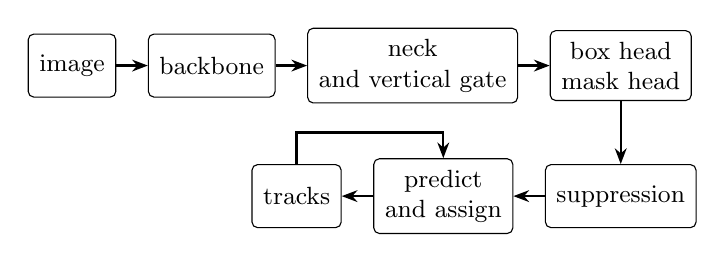
\begin{tikzpicture}[
  font=\small,
  box/.style={draw, rounded corners=2pt, align=center, inner sep=4pt, minimum height=8mm},
  arr/.style={-{Stealth[length=2mm]}, thick}
]
\node[box] (im) {image};
\node[box, right=4mm of im] (bb) {backbone};
\node[box, right=4mm of bb] (nk) {neck\\and vertical gate};
\node[box, right=4mm of nk] (hd) {box head\\mask head};
\node[box, below=8mm of hd] (nms) {suppression};
\node[box, left=4mm of nms] (trk) {predict\\and assign};
\node[box, left=4mm of trk] (id) {tracks};
\draw[arr] (im) -- (bb);
\draw[arr] (bb) -- (nk);
\draw[arr] (nk) -- (hd);
\draw[arr] (hd) -- (nms);
\draw[arr] (nms) -- (trk);
\draw[arr] (trk) -- (id);
\draw[arr] (id.north) -- ++(0,4mm) -| (trk.north);
\end{tikzpicture}
\caption{One frame, then the link to the previous frame. The loop on the right is the tracker. The thesis booking path stops at the masks and does not take that loop.}
\label{fig:pipe}
\end{figure}

\section{From the first YOLO to the crate segmenter}
\label{sec:line}

The family is a sequence of engineering choices on the same one-pass idea. Remembering which choice solved which defect keeps a deployment from turning every new release into a reason to restart.

YOLOv1 predicted two boxes per cell and one class vector per cell, and it trained with a sum of squared errors, taking the square root of width and height so that a large box did not dominate the loss~\cite{redmon2016yolo}. It was real-time on the hardware of 2016. It struggled with small objects and with two objects in one cell, which is exactly a stack of crates.

YOLOv2 introduced batch normalization, a higher input resolution, anchor boxes chosen by clustering, and a passthrough that stacked fine features into the detection map~\cite{redmon2017yolo9000}. The anchors are priors. They help when the dataset really does contain a few dominant shapes. They hurt when an anchor is a person-shaped prior and the object is a wide, short crate face.

YOLOv3 replaced the backbone with Darknet-53, predicted at three scales, and treated classes as independent logistics~\cite{redmon2018yolov3}. Three scales are the model's answer to ``the object might be 30 pixels or 300.'' A gate camera with a locked mount mostly sees one scale. The fine scale is still the one that can split two lips.

YOLOv4 assembled a CSPDarknet backbone, a spatial pyramid pooling block, a PANet neck, mosaic augmentation, and the complete-IoU loss~\cite{bochkovskiy2020yolov4,zheng2020diou}. Mosaic is a training trick: four images are pasted into one, so the batch contains objects at unusual positions. It is not a model of a forklift. A crate line should not assume that mosaic has taught the network what a half-occluded rank looks like, because the rear rank is not in the image at all. Depth has to come from a pallet record, which is the thesis's position and is unchanged by any detector release.

YOLOX discarded anchors, decoupled the head, and assigned positives with SimOTA~\cite{ge2021yolox}. YOLOv6 pursued a similar anchor-free industrial design~\cite{li2022yolov6}. YOLOv7 concentrated on training tricks that improve accuracy without raising the inference cost, and on an extended efficient layer aggregation network in the backbone~\cite{wang2023yolov7}. YOLOv8, the line the crate segmenter follows, is the Ultralytics anchor-free model with a decoupled head, a classification branch, a regression branch trained with complete IoU and a distributional box loss, and optional task heads for segmentation and pose~\cite{jocher2023yolov8}. YOLOv9's programmable gradient information and YOLOv10's attention to end-to-end inference without a separate suppression step are later points on the same curve~\cite{wang2024yolov9,wang2024yolov10}. They do not change the interface a tracker needs: a set of boxes with scores, produced per frame.

Two absences matter. Joseph Redmon stopped the original line at version 3. Everything after that is other groups reusing the name. A citation of ``YOLO'' without a version is not a specification. And no version in this list was trained on the gate. A deployment that starts from a public checkpoint trained on COCO~\cite{lin2014coco} still has to continue training on labeled gate frames if the lips, the plastic texture, and the six colors are to be reliable. This note does not report that training. The thesis does not either.

\section{Suppression, and when two crates become one box}
\label{sec:nms}

Dense heads emit far more boxes than there are crates. Non-maximum suppression is the cleanup. Sort the boxes of one class by score. Keep the best. Delete every remaining box whose IoU with the kept box exceeds a threshold. Repeat~\cite{girshick2015fast}. The threshold is a calibration choice. A high threshold lets two real crates both survive when their boxes overlap because of perspective. A low threshold deletes the second crate and the tally is short by one. Soft-NMS decays the score of the neighbor instead of deleting it, which is gentler when the overlap is legitimate~\cite{bodla2017softnms}. YOLOv10's training scheme tries to make the extras lose so completely that the cleanup can be omitted~\cite{wang2024yolov10}. Omitting it is safe only after the score distribution on the target images has been inspected. It is not safe by reputation.

On a stack, the dangerous overlap is vertical. Two identical faces with a faint lip between them produce two high scores whose boxes share a band of pixels. Equation~\eqref{eq:iou-shift} with a small $d$ gives a high IoU, and a strict threshold keeps one box. The vertical-feature gate is the baseline's attempt to make the lip strong enough that the two centers separate before suppression runs. Boundary refinement can clean a contour after the fact~\cite{kirillov2020pointrend}. Neither step is a tracker. A tracker that receives one merged box has one detection. It will follow that merge for as long as the merge persists, and it will not invent the missing crate. Association cannot repair a seam the detector never split.

Suppression also interacts with class labels. If amber and yellow are different classes, a box of each class will not suppress the other under the usual per-class rule. A single face that flickers between those two labels across frames will look, to a class-wise tracker, like two objects trading places. The color margin used in the thesis is a more honest signal than a hard label at that boundary: the prototypes of amber and yellow sit about $9.3^{\circ}$ apart, and a harsh illuminant confuses them. A tracker that keys identity on the color class will switch identifiers exactly on the pairs the color head finds hardest. Section~\ref{sec:modern} therefore treats color as a weak cue.

\section{Masks, centers, and the hand-off to a tracker}
\label{sec:mask}

A box is a poor summary of a crate that is partly hidden by the crate in front of it, and it is a poor summary of a lip. Instance segmentation returns the pixels. Mask R-CNN does this with a small convolutional head on each region of interest~\cite{he2017mask}. That is a second stage. YOLACT keeps the one-pass budget by predicting a set of mask prototypes for the whole image and a coefficient vector per detection. The mask is a linear combination of the prototypes, passed through a sigmoid and cropped to the box~\cite{bolya2019yolact}. YOLOv8-seg uses that pattern, typically with $32$ prototypes. YOLO-vf-seg uses it as well. The crop is important. Without it, a prototype that responds to a whole column of crates would paint every face in the column.

The center that a lattice counter wants is the first moment of the mask, not the center of the box. A box center drifts toward the empty part of the rectangle when the visible region is only the left half of a face. A mask center stays on the visible plastic. Tracking can use either point, but the two points are not interchangeable when the association gate is a few centimetres wide. A method that detects on boxes and counts on mask centers must say which point enters the Kalman filter. This note uses the box when the discussion is the classical SORT filter, because that is the point SORT was written for, and it uses the mask center when the discussion is the gate's metre lattice. Publishing a track identifier from one and a cell index from the other, without saying so, produces mismatches that look like detector failures.

The mask is also the only region a color measurement should average. Pixels outside it belong to a neighbor or to the dock. A tracker that crops a re-identification embedding from the box rather than from the mask will mix the two colors whenever the box crosses a lip. On this stack that mixture is common, because the boxes overlap by construction. If an appearance feature is used at all, it should be pooled inside the mask. The thesis already pools inside the mask for color. A tracking embedding can share that crop. It should not share the conclusion that two faces of the same color are the same crate.

\section{What a track is}
\label{sec:track}

A track is a hypothesis that a sequence of detections is one physical object. It stores an identifier, a motion state, an age, and a counter of how many frames have passed since the last matched detection. It may store an appearance vector. It does not store the truth. The identifier is a name the filter invented.

The standard way to build tracks from a detector is tracking-by-detection. Each frame is detected independently. A separate, usually much cheaper, step links the detections. SORT is the minimal version that still works: a Kalman filter per track, an IoU cost, and the Hungarian algorithm to pick a global assignment~\cite{bewley2016sort,kuhn1955hungarian}. DeepSORT adds an appearance distance and a matching cascade that prefers recently seen tracks~\cite{wojke2017deepsort}. Joint models such as CenterTrack predict, inside the detector, a vector from the current center to the previous center~\cite{zhou2020centertrack}. FairMOT shares a backbone between detection and a re-identification embedding~\cite{zhang2021fairmot}. The crate line does not need the joint models to understand the problem. It needs the vocabulary: prediction, gate, cost, assignment, birth, death.

Birth happens when a detection matches nothing. The new track is tentative until it has matched for a few frames, so a one-frame false positive does not become a crate. Death happens when a track has gone unmatched longer than a set age. Between birth and death the track can coast: the filter predicts a box even though the detector missed. Coasting is how a tracker fills a one-frame gap. It is also how a tracker invents a crate that has already left the image, if the age is longer than the gap. On a buffer of at most seven frames at $15\,\mathrm{Hz}$, the whole passage is under half a second. An age of thirty frames, copied from a pedestrian benchmark, is an age that never expires during the passage. The pallet would leave the gate still ``tracked.'' The age has to be chosen for this camera, not inherited from MOT17~\cite{milan2016mot16}.

Three published scores keep the language honest. MOTA combines misses, false positives, and identifier switches into one penalty~\cite{bernardin2008clear}. MOTP measures how well the matched boxes overlap, and it does not see a switch. IDF1 scores how much of a true object's life was kept under one identifier~\cite{ristani2016id}. HOTA separates detection accuracy from association accuracy so that a detector improvement is not mistaken for a tracker improvement~\cite{luiten2021hota}. This note quotes none of them as a result. There is no labeled passage. The scores are named so that a later measurement has somewhere to put its numbers, and so that a single ``tracking accuracy'' percentage is not asked to mean all four things.

\section{Predicting the next image}
\label{sec:kalman}

The Kalman filter is the linear estimator that updates a Gaussian state with a Gaussian measurement~\cite{kalman1960}. SORT applies it to a seven-dimensional state: the box center $(u,v)$, the area $s$, the aspect ratio $r$, and the velocities of the center and of the area. The aspect ratio is observed but not given a velocity. The picture is constant velocity in image coordinates. For the arithmetic, a two-dimensional slice is enough: horizontal position and horizontal velocity, in pixels and pixels per frame. The vertical slice is the same with its own numbers. Writing $\mathbf{x}=(u,\dot u)^{\mathsf T}$,
\begin{equation}
\mathbf{x}_{t|t-1} = F\mathbf{x}_{t-1|t-1},
\qquad
F = \begin{pmatrix} 1 & 1 \\ 0 & 1 \end{pmatrix},
\label{eq:predict}
\end{equation}
because the frame step has been absorbed into the unit of velocity. The covariance prediction is
\begin{equation}
P_{t|t-1} = F P_{t-1|t-1} F^{\mathsf T} + Q.
\label{eq:pcov}
\end{equation}
$Q$ is the process noise. It is the filter's admission that a forklift does not hold a perfectly constant speed. A driver who slows at the beam is exactly this term. If $Q$ is too small, the filter trusts the old velocity and predicts the crate into the next cell. If $Q$ is too large, the prediction is so wide that it no longer gates anything.

The measurement is the detected center, $z_t = H\mathbf{x} + \mathrm{noise}$, with $H=(1\ 0)$. The update pulls the prediction toward $z_t$ by a gain $K$:
\begin{align}
S &= H P_{t|t-1} H^{\mathsf T} + R, \nonumber\\
K &= P_{t|t-1} H^{\mathsf T} S^{-1}, \nonumber\\
\mathbf{x}_{t|t} &= \mathbf{x}_{t|t-1} + K\bigl(z_t - H\mathbf{x}_{t|t-1}\bigr), \nonumber\\
P_{t|t} &= (I - KH)\,P_{t|t-1}.
\label{eq:update}
\end{align}
$R$ is the measurement noise. On this camera it is the jitter of the detected center, in pixels, not the uncertainty of the count.

A numerical step makes the matrices honest. Take a slow pass, derived in Section~\ref{sec:passage}, of about $56$ pixels per frame. Suppose the filter currently believes $\mathbf{x}=(400, 56)^{\mathsf T}$ and
\[
P = \begin{pmatrix} 9 & 0 \\ 0 & 4 \end{pmatrix},
\qquad
Q = \begin{pmatrix} 1 & 0 \\ 0 & 0.25 \end{pmatrix}.
\]
These two matrices are choices used to show the arithmetic. They are not fitted to footage. Then $FPF^{\mathsf T}+Q$ evaluates to
\[
P_{t|t-1} = \begin{pmatrix} 14 & 4 \\ 4 & 4.25 \end{pmatrix}.
\]
The predicted center is $456$. With $R=9$ and a detection at column $458$, the innovation is $2$ pixels and $S=14+9=23$. The gain is $(14/23,\ 4/23)^{\mathsf T}$, about $(0.609,\ 0.174)^{\mathsf T}$. The updated state is about $(457.2,\ 56.3)^{\mathsf T}$. The filter accepted most of the two-pixel disagreement and added a third of a pixel per frame to the velocity. Had the detection landed at $500$, the innovation would be $44$ pixels. The same gain would shove the velocity by about $7.7$ pixels per frame in a single step. That is why a gate belongs in front of the update. A detection that far from the prediction is either a different crate or a merged seam, and it should not be allowed to rewrite the velocity before the assignment has accepted it.

Image coordinates are the wrong place for the constant-velocity assumption when the load also approaches the camera. Approach changes scale. A crate that is constant in metres grows in pixels, and the area component of the SORT state acquires a velocity that is really a change of standoff. The gate specification is a side view at about $2.5\,\mathrm{m}$, looking at the face as the forklift travels across the field of view. The calculation in this note assumes that pass: translation along the face, scale nearly fixed. A turn in which the forks point at the camera needs the homography already used to put centers into metres, and then a constant-velocity model in metres rather than in pixels. The Kalman equations do not change. $F$ is applied to $(X,\dot X)$ on the rectified face. That is the motion model that matches the lattice.

\section{Assigning detections to tracks}
\label{sec:assign}

Prediction produces a box for every living track. Detection produces a box for every object the network will admit. The assignment is a bijection between a subset of the tracks and a subset of the detections. Tracks left over may coast or die. Detections left over may start tracks.

The cost of pairing track $i$ with detection $j$ in SORT is the complement of the overlap,
\begin{equation}
C_{ij} = 1 - \mathrm{IoU}(\hat{B}_i, B_j),
\label{eq:cost}
\end{equation}
and the pair is forbidden when the IoU falls below a threshold. The Hungarian algorithm finds the permutation of allowed pairs with the smallest total cost~\cite{kuhn1955hungarian}. Greedy matching, taking the best pair and removing its row and column, is close when one pair is obvious and wrong when two tracks compete for two nearby detections. On a regular stack the centers are a pitch apart, so the competition is real. The global assignment is the one that matches the lattice.

Consider three tracks whose predicted centers, in pixels along the row, sit at $100$, $322$, and $544$. That spacing is one face: $0.40\,\mathrm{m}$ at $1.8\,\mathrm{mm}$ per pixel is $222$ pixels, and $100+222=322$. The faces are $222$ pixels wide. Three detections arrive at $104$, $380$, and $548$. Using~\eqref{eq:iou-shift}:

\begin{center}
\begin{tabular}{lccc}
\toprule
 & det.\ at $104$ & det.\ at $380$ & det.\ at $548$ \\
\midrule
track $100$ & $0.965$ & $0$ & $0$ \\
track $322$ & $0$ & $0.586$ & $0$ \\
track $544$ & $0$ & $0$ & $0.965$ \\
\bottomrule
\end{tabular}
\end{center}

The zeros are overlaps of boxes whose center gap exceeds the width. The middle value is $(222-58)/(222+58)=164/280=0.586$. It clears a gate of $0.5$ and fails a gate of $0.8$. The unique allowed matching at a gate of $0.5$ pairs each track with the detection in its own column of the table. Raise the middle detection's miss so that it is absent, and the middle track coasts. Drop an extra detection halfway between the first and the second, and its IoU with both neighbors should be inspected before it is allowed to birth a track: a false positive between two real lips is the usual source of a short-lived identifier.

DeepSORT replaces the bare IoU gate with a Mahalanobis gate on the Kalman covariance, and it adds a cosine distance between appearance embeddings to the cost~\cite{wojke2017deepsort}. The Mahalanobis gate is the right idea when some tracks are uncertain and others are not. A young track with a large $P$ may accept a detection that an old, tight track must reject. A fixed IoU threshold cannot say that. The cascade, matching confirmed tracks before tentative ones, exists so that a new false detection does not steal an identifier from a crate that has been followed for several frames.

The cost can be written in metres on the rectified face, which is the coordinate already used for counting. Let $\mathbf{p}_i$ be the predicted centre and $\mathbf{q}_j$ the detected mask centre, both in metres. A squared distance
\begin{equation}
C_{ij} = (p_{i,x}-q_{j,x})^2 + (p_{i,y}-q_{j,y})^2
\label{eq:costm}
\end{equation}
is forbidden when it exceeds $(0.20\,\mathrm{m})^2$, half a cell of the $0.40\,\mathrm{m}$ pitch. Half a cell is the same radius the thesis uses as a refusal test on the origin residual. Reusing it as an association gate means a detection that would snap to a different cell is not allowed to update this track. The tracker and the lattice then disagree in a controlled way: they disagree when the detection is more than half a pitch from the prediction, and that disagreement can be logged instead of being averaged away.

\section{Appearance, low scores, and camera motion}
\label{sec:modern}

Identical crates are the case appearance matching was not designed for. A person re-identification embedding works because clothing, hair, and build differ. Two amber crates from the same brewery differ by a scuff and a glare spot. A cosine distance between their embeddings is small for the right reason and also small for the wrong neighbor. Using that distance as a large term in $C_{ij}$ will confidently associate a track with the adjacent crate of the same color when the motion cue was the one that knew the difference. The safe order on this line is the opposite of the pedestrian default: motion first, appearance only as a tie break inside the motion gate, and color class not as an identity at all.

ByteTrack's contribution is to stop throwing low-score boxes away before association~\cite{zhang2022bytetrack}. The detector's list is split by a high threshold and a low threshold. Tracks match the high-score boxes first. Unmatched tracks then match the low-score boxes, typically by IoU alone, with no appearance term, because a box that barely survived the detector is a bad place to compute an embedding. Unmatched high-score boxes start new tracks. Low-score boxes that match nothing are discarded. The procedure recovers a crate whose score dipped because of blur, a shadow, or a partial lip, without promoting every speck to an identity. It assumes the low-score box is still in the right place. A merged seam that is low-scoring and shifted by half a face will be accepted by a wide IoU gate and will drag the track. The second-stage gate should stay at the half-cell radius of~\eqref{eq:costm}, not at the loose overlap that pedestrian trackers tolerate.

BoT-SORT adds a compensation for camera motion before the IoU is computed, and it mixes IoU with a re-identification cosine distance~\cite{aharon2022botsort}. Camera motion matters when the gate camera is bumped or when an auto-exposure crop changes. It matters much less when the camera is bolted and the only motion is the forklift. Compensating a bolted camera with an estimated homography every frame can remove a real crate displacement if the estimator locks onto the stack instead of onto the dock. The dock, the floor mark, and the beam housing are the background. The stack is not. A compensation estimated from points on the crates will cancel the motion the tracker is supposed to follow.

OC-SORT observes that a Kalman filter which coasts through an occlusion and is then corrected by one new detection can be pulled off the true velocity, and it rebuilds the velocity from the last two actual observations instead of from the coasted state~\cite{cao2023ocsort}. The failure it targets is visible in the numerical update above. A single bad innovation, applied with a healthy gain, changes $\dot u$. If the miss lasted several frames, the coasted position is where the old velocity put it, and the first new detection may be a different crate that entered the gate. Recomputing the velocity from the last real matches limits the damage. On a passage shorter than seven frames there are not many observations to recompute from. OC-SORT's impulse still applies in miniature: do not let the first detection after a miss rewrite the speed that the frames before the miss had agreed on, unless the spatial gate accepts it.

CenterTrack and FairMOT fold the link into the network~\cite{zhou2020centertrack,zhang2021fairmot}. The detector emits an offset to the previous frame, or an embedding trained to be stable across frames. Both can outperform a bolted-on Kalman filter when the training set contains the same kind of occlusion as the test set. A public pedestrian tracker, dropped onto crates without that training, has not received the benefit those papers measured. The honest implementation path for the gate is the external filter of this note, fed by YOLO-vf-seg, until a labeled set of passages exists. Training a joint tracker on COCO person identities will not teach it the pitch of a crate.

\begin{table}[t]
\centering
\small
\begin{tabular}{llp{6.6cm}}
\toprule
Method & Link & What it will not do on identical crates \\
\midrule
SORT & Kalman, IoU, Hungarian & Above $3\,\mathrm{m\,s^{-1}}$ the neighbor out-overlaps the crate. \\
DeepSORT & Motion gate plus embedding & The embedding confuses equal colors. \\
ByteTrack & High scores, then low scores & A shifted low-score seam can still attach. \\
BoT-SORT & Camera motion plus embedding & Motion compensation can lock onto the stack. \\
OC-SORT & Velocity from real observations & A seven-frame passage gives it little history. \\
\bottomrule
\end{tabular}
\caption{Association methods as they apply to a stack of similar faces. The remarks are consequences of the methods, not scores on a crate dataset.}
\label{tab:trackers}
\end{table}

\section{How far the stack moves between two frames}
\label{sec:passage}

The gate specification fixes the quantities a tracker would be built from. The camera runs at $15\,\mathrm{Hz}$, so the frame interval is $1/15\,\mathrm{s}$. The exposure is at most $2\,\mathrm{ms}$, which keeps smear small: at $1.5\,\mathrm{m\,s^{-1}}$ the load moves $3\,\mathrm{mm}$ during the exposure, about two pixels at $1.8\,\mathrm{mm}$ per pixel. Smear of that size blurs a lip. It does not, by itself, move a center into the next cell. The motion that the tracker must absorb is the motion between frames, which is thirty times larger than the motion during the exposure.

At a lateral speed $v$,
\begin{equation}
\Delta x = v\cdot \frac{1}{15}.
\label{eq:dx}
\end{equation}
At $1.5\,\mathrm{m\,s^{-1}}$, $\Delta x = 0.100\,\mathrm{m}$, which is $56$ pixels and a quarter of the $0.40\,\mathrm{m}$ face. Equation~\eqref{eq:iou-shift} then gives
\[
\mathrm{IoU} = \frac{0.40-0.10}{0.40+0.10} = 0.60
\]
if the predicted box was left where the previous detection was. A gate of $0.5$ still matches. A gate of $0.7$, copied from a careful pedestrian setup, does not. At $5\,\mathrm{m\,s^{-1}}$, $\Delta x = 0.333\,\mathrm{m}$ and the same unpredicted overlap is
\[
\mathrm{IoU} = \frac{0.40-0.333}{0.40+0.333} = 0.091.
\]
No reasonable IoU threshold matches a crate to its own previous box at that speed. The comparison that does match is the previous box of the neighbor. The neighbor sits one pitch, $0.40\,\mathrm{m}$, ahead. After a shift of $0.333\,\mathrm{m}$ the residual to that neighbor is $0.067\,\mathrm{m}$, and
\[
\mathrm{IoU} = \frac{0.40-0.067}{0.40+0.067} = 0.713.
\]
The crate overlaps its own history at $0.091$ and its neighbor's history at $0.713$. A Hungarian step on IoU will hand every identifier one cell down the stack, birth a track at the leading edge, and kill a track at the trailing edge. The swap is not a bug in the solver. It is the cost the solver was given.

The two overlaps are equal when the shift is half a pitch. Half of $0.40\,\mathrm{m}$ in one frame of $1/15\,\mathrm{s}$ is a lateral speed of $3\,\mathrm{m\,s^{-1}}$. Below that speed, overlap with one's own previous box is the larger of the two. Above it, the neighbor wins, and a tracker that has not yet got a velocity will rename the stack on every frame. SORT initializes those velocities at zero~\cite{bewley2016sort}, so the first assignment really is an assignment against the previous boxes, not against a prediction. Waiting for the filter to ``learn the speed'' does not help if the first pairing already attached each track to the wrong crate. The speed it learns is then the speed of the wrong pairing, which is a small residual, and the identifiers walk.

Table~\ref{tab:motion} collects the two speeds. The pixel column uses $1.8\,\mathrm{mm}$ per pixel from the specification of a $1280$-pixel-wide view at the working standoff. Both rows are arithmetic, not measurements of a forklift that was filmed.

\begin{table}[t]
\centering
\small
\begin{tabular}{lrrrr}
\toprule
Lateral speed & Shift per frame & Pixels & IoU if unpredicted & Fraction of one cell \\
\midrule
$1.5\,\mathrm{m\,s^{-1}}$ & $0.100\,\mathrm{m}$ & $56$ & $0.60$ & $0.25$ \\
$5.0\,\mathrm{m\,s^{-1}}$ & $0.333\,\mathrm{m}$ & $185$ & $0.091$ & $0.83$ \\
\bottomrule
\end{tabular}
\caption{Motion of one face between consecutive frames at $15\,\mathrm{Hz}$, computed from the gate specification. The IoU column compares a box to the same box shifted by that motion, with no Kalman prediction.}
\label{tab:motion}
\end{table}

The vertical velocity is near zero in a pure lateral pass, so a row of the stack stays in its row. That is why a cost that adds $(p_y-q_y)^2$ is informative: a detection that has jumped up by most of $0.28\,\mathrm{m}$ is a different tier, even if its horizontal position matches a coasted track. Perspective and a change of standoff bend this. A load that approaches by a few tens of centimetres grows in the image and the upper tiers move faster in pixels than the lower tiers, because they are farther from the camera's horizontal axis. A single image-wide velocity is then the wrong model. Per-track velocities, which SORT already keeps, absorb a smooth version of that shear. They do not absorb a wrong homography. If the metre conversion is off by a scale factor, every track is still internally consistent in pixels and the lattice is consistently wrong. Tracking health is not a calibration check.

Blur enters the detector before it enters the filter. The thesis models a detection probability that falls with a blur variable and is lower on the bottom and top rows than on the middle rows. A tracker sees the consequence as a miss. Coasting can hold the identifier across one missed frame of a slow pass, because the next detection still falls inside the half-cell gate around the prediction. On the fast pass, a miss of two frames is a displacement of $0.67\,\mathrm{m}$, more than a cell and a half. A coasted track and the reappearing crate no longer satisfy~\eqref{eq:costm}. The correct behavior is a new identifier, not a long coast that leaps a cell and attaches to whoever now occupies the predicted point. Short age, tight spatial gate, no appearance override: those three settings follow from the table, without any filmed sequence.

\section{One speed for the whole face}
\label{sec:rigid}

The stack is a rigid body for the fraction of a second it is in front of the camera. The crates do not pass each other. There is therefore one horizontal shift $s$ between frame $t$ and frame $t+1$, not one independent mystery per crate. Estimating that single shift before any identifier is updated removes the neighbor trap.

Let the mask centers on the rectified face be $x_1,\ldots,x_m$ and $y_1,\ldots,y_n$, in metres along the row. A candidate shift $s$ is scored by how many centers it explains:
\begin{equation}
N(s) = \text{maximum matching of pairs with } |x_i + s - y_j| \le 0.20\,\mathrm{m}.
\label{eq:inliers}
\end{equation}
The threshold is again half a cell, so a candidate that is off by a full pitch cannot claim the same pair. The shift that is kept is the one with the largest $N(s)$. It can be found by testing the observed differences $y_j-x_i$, because an optimal shift can always be moved until one pair sits on top of another without losing inliers, or by scanning $s$ from $0$ to one pitch in steps of a centimetre. There are only a few dozen centers. The scan is cheaper than the segmenter by a large factor.

On the fast numbers, $s=0.333\,\mathrm{m}$ puts every repeated crate inside the half-cell and $N(s)$ equals the number of crates seen in both frames. The off-by-one candidate $s=0.333-0.40=-0.067\,\mathrm{m}$ explains only the crates that are not at the end of the row: each end falls off. A row of four faces therefore scores $4$ at the true shift and $3$ at the shifted one. The true shift wins. A row of two faces can tie, because each hypothesis explains one pair and leaves one over. The gate sees columns of two to four and rows of two to six, so the face as a whole, not one row in isolation, is the set that should enter~\eqref{eq:inliers}. Using a single row of two is the configuration in which the rigid estimate is allowed to abstain and the passage is marked unidentified rather than renamed.

Once $s$ is chosen, every track that was matched through it is given velocity $s$ per frame, and the Kalman filter continues from there. The next frame predicts $x+2s$ if the speed holds. Association returns to the half-cell gate around that prediction. A crate that truly moved with the pallet falls inside the gate. A false detection on the dock does not, unless the dock point happened to lie half a cell from some crate after the same shift. Those leftovers fail the birth rule when a second frame does not support them at the same speed.

This is not a claim that a filmed forklift holds $s$ constant to a centimetre. Braking at the beam is a change of $s$. Re-estimating $s$ every frame, from the tracks' predicted centers to the new detections, follows a smooth brake. What the rigid step forbids is a solution in which neighboring crates take opposite velocities so that an IoU accident can persist. Opposite velocities are physically available to pedestrians. They are not available to crates bolted by gravity into one pallet.

\section{Five frames of one crate}

The slow pass is the one in which a per-track filter is easy to watch, because $0.10\,\mathrm{m}$ per frame never reaches the neighbor. Take a single face whose true centers at $15\,\mathrm{Hz}$ are $1.00$, $1.10$, $1.20$, $1.30$, $1.40$ metres, and suppose the detector returns all of them except the fourth. The account below is the rule of Sections~\ref{sec:kalman} and~\ref{sec:rigid} applied to those five numbers. It is an example, not a log.

Frame 1 has no living track. The detection at $1.00$ starts a tentative track with unknown speed. Frame 2, together with every other detection on the face, yields $s=0.10\,\mathrm{m}$. The tentative track matches the detection at $1.10$, becomes confirmed, and stores velocity $0.10\,\mathrm{m}$ per frame. Frame 3 predicts $1.20$. The detection is there. The innovation is zero if the center is exact, and the velocity is unchanged. Frame 4 predicts $1.30$. The detector misses. The track coasts: the state is not updated, the miss counter becomes one, and no box is added to any tally. Frame 5 predicts $1.40$. The detection returns. The miss counter clears. The identifier that was born at $1.00$ is the identifier at $1.40$.

Two changes break the story in ways the rules already name. If frame 5 had come back at $1.55$, the residual to the prediction would be $0.25\,\mathrm{m}$, outside the half-cell, and the old track would not absorb it. If frame 4 and frame 5 were both missing, the miss counter would hit two and the track would die rather than leap onward. If the same five centers were replaced by the fast step $0.333\,\mathrm{m}$ and the rigid estimate were skipped, frame 2 would attach the detection to the previous neighbor, as Section~\ref{sec:passage} calculated, and the calm update of frame 3 would never be about the same crate.

A second crate one pitch away runs the same frames at $1.40$, $1.50$, $1.60$, $1.70$, $1.80$. The rigid shift is estimated once, from both crates and the rest of the face. Each track then consumes only the detection inside its own gate. The two identifiers do not cross. That separation is the entire content of image tracking on a lattice: one shared motion, then a private gate per object.

\section{The loss that places the box}

The tracker never sees the loss. The detector's errors, which the tracker must live with, are the errors the loss chose to punish. A short account belongs with the detector half of this note.

YOLOv1 added squared errors on the box center, on the square roots of width and height, on the confidence, and on the class probabilities, with a larger weight on coordinates than on empty cells~\cite{redmon2016yolo}. Squared error treats a one-pixel miss the same whether the box is tight or loose, and it does not know what overlap is. Later heads train the box with a loss written on the overlap itself. Complete IoU is the form used by YOLOv4 and kept, with a distributional refinement, in the Ultralytics line~\cite{zheng2020diou,bochkovskiy2020yolov4}. For a predicted box $B$ and a true box $B^{\star}$,
\begin{equation}
\mathcal{L}_{\mathrm{CIoU}} = 1 - \mathrm{IoU}(B,B^{\star}) + \frac{\rho^{2}(b,b^{\star})}{c^{2}} + \alpha v,
\label{eq:ciou}
\end{equation}
where $b$ and $b^{\star}$ are the centers, $\rho$ is their Euclidean distance, $c$ is the diagonal of the smallest box that contains both rectangles, and
\begin{equation}
v = \frac{4}{\pi^{2}}\left(\arctan\frac{w^{\star}}{h^{\star}} - \arctan\frac{w}{h}\right)^{2}
\label{eq:var}
\end{equation}
measures the difference of aspect ratios. The weight $\alpha$ grows when the overlap is already good, so the aspect term matters most for boxes that are in the right place and the wrong shape. On a crate face the true aspect is $0.40/0.28$. A box that covers two stacked faces is about twice as tall. Equation~\eqref{eq:var} sees that. It does not, by itself, split the seam. It only tells a box that already overlaps both faces that its shape is expensive.

A distributional box loss, of the kind introduced for generalized focal loss and used in the YOLOv8 regression branch, stops predicting a single distance to each side and instead predicts a small discrete distribution over that distance~\cite{li2020gfl}. The training target puts its mass on the two bins that bracket the true distance, and the decoded distance is the expected value of the distribution. The practical effect is a box whose boundary can express uncertainty. A lip that is soft under blur becomes a wider distribution rather than a confident edge in the wrong place. The tracker should read the decoded box, which is what suppression and the Kalman filter expect. Reading the mode of one bin, or treating the spread as a change in the crate's size, mixes a training detail into the motion state.

Class loss is a separate term, cross-entropy or a binary logistic loss on the labels the assignment marked positive. It is the term that learns ``crate'' versus ``dock.'' It is not the term that separates amber from yellow inside a mask. That separation, in the thesis, is the chromatic head on pixels the mask already selected. Training the detector's class branch on the six colors as well is possible, and it would give the tracker a label. Section~\ref{sec:modern} is why that label is a weak identity. The loss can be right on average and still flip two neighboring colors from frame to frame when the illuminant moves.

What the loss does not contain is any term from the previous frame. YOLO is trained, in the standard setup, on still images. A box that jumps by half a cell between two real frames is not an error the detection loss ever saw, unless the training set was built from video and the assignment was told about time. The offsets inside CenterTrack are one way to add that term~\cite{zhou2020centertrack}. They are not in YOLO-vf-seg. The smoothness of a track is imposed after the fact, by the gate and the rigid shift, and it should stay there until a video loss is actually trained.

\section{What tracking must not be asked to count}
\label{sec:count}

A track answers a question of identity. A count answers a question of cardinality. They share an input, the detector list, and they fail in different directions.

The thesis counter rectifies the front face, snaps mask centers to the known pitch, fills an empty cell only when at least two orthogonal neighbors support it, and multiplies by a depth reading. It does this on the sharpest frame in the buffer. A five-frame union of occupied cells, which is the naive way to ``use tracking'' as a count, over-filled under the same Monte Carlo model: holes were repaired, and cells that were empty for a real reason were also filled. The specified software therefore keeps no identity across frames. That negative result is about booking a union. It is not a proof that identities are useless for every other question an operator might ask.

There are questions a tracker can answer and a single-frame lattice cannot. Whether the face now in front of the camera is the same face that tripped the beam, or a second pallet that arrived before the buffer closed. Whether a crate that was missing on the sharpest frame was present on the frames around it, which is a cue to send the passage to a person rather than to invent the crate. Whether one detection jumped by half a cell between frames, which is a cue that two lips were merged and then split. All three are checks. None of them is a term in the sum that becomes the booked count. The moment a coasted track is added into that sum, the system has reintroduced the union it already measured as worse.

The practical arrangement, if a later deployment turns the tracker on, is a parallel record. YOLO-vf-seg runs on each kept frame, as the thesis specifies. The sharpest frame still goes to the color head and to the lattice, and that lattice result is the number that is booked. In parallel, the assignment of Section~\ref{sec:assign} maintains identifiers over the buffer. The record stores the number of identifier switches, the number of tracks that were alive at the end of the passage, and the number of frames each booked cell was detected on. A cell detected once in seven frames is a weaker cell than a cell detected seven times, even when both snap to the same place. Storing that multiplicity does not change the count. It tells the operator which lines of the tally the detector barely supported. Acting on it by adding the coasted-only cells would change the count, and this note does not recommend that action.

False positives need the same discipline. A reflection on the floor that survives one frame will fail the birth rule if birth requires two matches. A reflection that tracks the forklift, because it is a specular patch moving at $v$, will be born and will follow the pallet. Motion consistency cannot reject it. Position can. A track whose rectified center falls outside the face that the lattice just estimated is not a crate, however smooth its velocity. The lattice, not the tracker, knows where the face is.

Color stays on the detection, not on the identifier. A track may display the color of its latest matched mask, together with the margin. It should not vote a color over the passage and then overwrite a low-margin frame with a high-margin neighbor's vote, because the neighbor may be the adjacent amber crate and the frame may be the yellow one. The chromatic head is per mask for that reason. Temporal smoothing of a feature is reasonable only inside one identifier and only among masks whose margins all cleared the abstention line. Smoothing across an identifier switch mixes the two faces the switch had just separated.

\section{A short implementation order}

The pieces above fit into one process beside the process the thesis already specifies. The order is the order of the data, and each step has a reason to be where it is.

The trigger opens and the camera writes a buffer at $15\,\mathrm{Hz}$, with the exposure held at or below $2\,\mathrm{ms}$ and the white balance locked. Locking the balance does not make color trivial, but it stops the camera from introducing a second, unknown illuminant change on top of the dock lighting. Frames that fail a brightness check are dropped before the detector, because a black frame has no business updating a velocity.

On each kept frame the segmenter emits boxes, scores, and masks. Suppression runs with a threshold that was chosen on labeled frames, not copied from a default of $0.7$ and forgotten. Mask centers are computed and converted to metres with the same homography the lattice uses. The Kalman filter predicts every living track to this time. On the first pair of frames, and again whenever the speed may have changed, one rigid shift is estimated by~\eqref{eq:inliers} and written into the matched tracks before any per-crate IoU is trusted. Association then uses~\eqref{eq:costm} inside a half-cell gate, high-score masks first and low-score masks second, with no appearance term outside the gate. Accepted matches update the filter. Unmatched high-score masks become tentative tracks. A tentative track that matches on the next frame is confirmed. A track that has been unmatched for two frames dies. Two frames at the fast speed of Table~\ref{tab:motion} are already more than a cell of coasting; a longer life would attach the track to a different crate.

When the trigger closes, the frame with the highest median color margin is sent to the lattice and to the color head, alone. The tracker contributes the diagnostic counts and then drops its state. Carrying identifiers from one pallet to the next is a bug: the next forklift is not the same object, even if it enters at the image position where the last one left.

Nothing in that order has been timed on the gate PC, and nothing in it has been scored with MOTA, IDF1, or HOTA. The timing claim that is safe to repeat is the one the thesis already makes about the segmenter: it is the heavy step, and the filter and the assignment are not. A few dozen boxes and a $7$-frame life do not stress a Hungarian solver. If the frame period is missed, the remedy is a smaller segmenter, not the deletion of the spatial gate.

\section{A template tracker is a different tool}

Image tracking is also the name of a second, older task: follow one region that a person marked in the first image, with no class and no list of other objects. Correlation filters such as MOSSE and the kernelized correlation filter learn a small template of that region and locate it in the next image by a convolution in the Fourier domain~\cite{bolme2010mosse,henriques2015kcf}. Siamese trackers learn an embedding in which the marked object matches itself across frames and does not match the background~\cite{bertinetto2016siamfc}. They are fast, and they are the wrong instrument for a stack.

A template tracker does not propose crates. It follows the patch it was given. Point it at one amber face and it may stay on that face while the forklift crawls, and it will not notice the twelve faces around it. Point it at a lip and the template is a horizontal edge that looks like every other lip. The update of the template, which is how these methods survive a slow change of appearance, will drink in the neighbor as soon as the original face moves by a quarter of its width. On the fast pass of Table~\ref{tab:motion} the patch has moved $185$ pixels, which is most of the face, and a search window sized for a pedestrian's step will not contain it.

YOLO's list is what makes the stack countable: every face that cleared suppression, each with a box, a score, and a mask. The tracker in this note does not replace that list with a template. It links lists. The template methods remain appropriate for a different request, a person drawing one box around a single crate they want followed through a turn. That request is not the gate's request. The gate's request is the whole face, found again in every frame, with identifiers that do not walk from crate to crate.

\section{Closing}

YOLO, in the form used on this line, is a one-pass instance segmenter. A cross-stage backbone and a feature pyramid build the maps, a vertical gate emphasizes the horizontal lips, a decoupled head emits boxes, and a prototype assembly emits masks. Suppression reduces the dense list to one box per object the threshold will allow. The mask center is the point a lattice can snap. None of those steps looks at the previous frame.

Image tracking begins at the next step. A Kalman filter predicts each living object with a constant-velocity model, an assignment with a half-cell gate decides which new mask continues which identity, low-score masks get a second chance only inside that gate, and birth and death are kept short because the passage itself is short. Appearance embeddings and color labels are weak on a stack of identical faces, so they do not get to overrule the geometry. At $1.5\,\mathrm{m\,s^{-1}}$ an unpredicted box still overlaps its predecessor at $0.60$. At $5\,\mathrm{m\,s^{-1}}$ that overlap falls to $0.091$ and the overlap with the previous neighbor rises to $0.713$. The association that survives the fast pass is a single rigid shift of the whole face, followed by a private gate per crate.

The booked count stays the single-frame lattice times the depth reading. The tracker can sit beside that count and report how steadily each cell was seen. It must not add its coasted boxes into the tally. Identity and cardinality answer different questions, and the passage is short enough that confusing them moves the number by a cell.

\begin{thebibliography}{99}
\bibitem{redmon2016yolo} J.~Redmon, S.~Divvala, R.~Girshick, and A.~Farhadi, ``You Only Look Once: Unified, real-time object detection,'' in \emph{CVPR}, 2016.
\bibitem{redmon2017yolo9000} J.~Redmon and A.~Farhadi, ``YOLO9000: Better, faster, stronger,'' in \emph{CVPR}, 2017.
\bibitem{redmon2018yolov3} J.~Redmon and A.~Farhadi, ``YOLOv3: An incremental improvement,'' arXiv:1804.02767, 2018.
\bibitem{bochkovskiy2020yolov4} A.~Bochkovskiy, C.-Y.~Wang, and H.-Y.~M.~Liao, ``YOLOv4: Optimal speed and accuracy of object detection,'' arXiv:2004.10934, 2020.
\bibitem{ge2021yolox} Z.~Ge, S.~Liu, F.~Wang, Z.~Li, and J.~Sun, ``YOLOX: Exceeding YOLO series in 2021,'' arXiv:2107.08430, 2021.
\bibitem{li2022yolov6} C.~Li \emph{et al.}, ``YOLOv6: A single-stage object detection framework for industrial applications,'' arXiv:2209.02976, 2022.
\bibitem{wang2023yolov7} C.-Y.~Wang, A.~Bochkovskiy, and H.-Y.~M.~Liao, ``YOLOv7: Trainable bag-of-freebies sets new state-of-the-art for real-time object detectors,'' in \emph{CVPR}, 2023.
\bibitem{jocher2023yolov8} G.~Jocher, A.~Chaurasia, and J.~Qiu, ``Ultralytics YOLO,'' software, 2023.
\bibitem{wang2024yolov9} C.-Y.~Wang, I.-H.~Yeh, and H.-Y.~M.~Liao, ``YOLOv9: Learning what you want to learn using programmable gradient information,'' arXiv:2402.13616, 2024.
\bibitem{wang2024yolov10} A.~Wang \emph{et al.}, ``YOLOv10: Real-time end-to-end object detection,'' arXiv:2405.14458, 2024.
\bibitem{lin2014coco} T.-Y.~Lin \emph{et al.}, ``Microsoft COCO: Common objects in context,'' in \emph{ECCV}, 2014.
\bibitem{lin2017fpn} T.-Y.~Lin, P.~Dollár, R.~Girshick, K.~He, B.~Hariharan, and S.~Belongie, ``Feature pyramid networks for object detection,'' in \emph{CVPR}, 2017.
\bibitem{he2016resnet} K.~He, X.~Zhang, S.~Ren, and J.~Sun, ``Deep residual learning for image recognition,'' in \emph{CVPR}, 2016.
\bibitem{wang2020cspnet} C.-Y.~Wang \emph{et al.}, ``CSPNet: A new backbone that can enhance learning capability of CNN,'' in \emph{CVPR Workshops}, 2020.
\bibitem{liu2018panet} S.~Liu, L.~Qi, H.~Qin, J.~Shi, and J.~Jia, ``Path aggregation network for instance segmentation,'' in \emph{CVPR}, 2018.
\bibitem{hou2021coordatt} Q.~Hou, D.~Zhou, and J.~Feng, ``Coordinate attention for efficient mobile network design,'' in \emph{CVPR}, 2021.
\bibitem{zheng2020diou} Z.~Zheng \emph{et al.}, ``Distance-IoU loss: Faster and better learning for bounding box regression,'' in \emph{AAAI}, 2020.
\bibitem{li2020gfl} X.~Li \emph{et al.}, ``Generalized focal loss: Learning qualified and distributed bounding boxes for dense object detection,'' in \emph{NeurIPS}, 2020.
\bibitem{ren2015faster} S.~Ren, K.~He, R.~Girshick, and J.~Sun, ``Faster R-CNN: Towards real-time object detection with region proposal networks,'' in \emph{NeurIPS}, 2015.
\bibitem{girshick2015fast} R.~Girshick, ``Fast R-CNN,'' in \emph{ICCV}, 2015.
\bibitem{bodla2017softnms} N.~Bodla, B.~Singh, R.~Chellappa, and L.~S.~Davis, ``Soft-NMS: Improving object detection with one line of code,'' in \emph{ICCV}, 2017.
\bibitem{he2017mask} K.~He, G.~Gkioxari, P.~Dollár, and R.~Girshick, ``Mask R-CNN,'' in \emph{ICCV}, 2017.
\bibitem{bolya2019yolact} D.~Bolya, C.~Zhou, F.~Xiao, and Y.~J.~Lee, ``YOLACT: Real-time instance segmentation,'' in \emph{ICCV}, 2019.
\bibitem{kirillov2020pointrend} A.~Kirillov, Y.~Wu, K.~He, and R.~Girshick, ``PointRend: Image segmentation as rendering,'' in \emph{CVPR}, 2020.
\bibitem{bewley2016sort} A.~Bewley, Z.~Ge, L.~Ott, F.~Ramos, and B.~Upcroft, ``Simple online and realtime tracking,'' in \emph{ICIP}, 2016.
\bibitem{wojke2017deepsort} N.~Wojke, A.~Bewley, and D.~Paulus, ``Simple online and realtime tracking with a deep association metric,'' in \emph{ICIP}, 2017.
\bibitem{zhang2022bytetrack} Y.~Zhang \emph{et al.}, ``ByteTrack: Multi-object tracking by associating every detection box,'' in \emph{ECCV}, 2022.
\bibitem{aharon2022botsort} N.~Aharon, R.~Orfaig, and B.-Z.~Bobrovsky, ``BoT-SORT: Robust associations multi-pedestrian tracking,'' arXiv:2206.14651, 2022.
\bibitem{cao2023ocsort} J.~Cao, J.~Pang, X.~Weng, R.~Khirodkar, and K.~Kitani, ``Observation-centric SORT: Rethinking SORT for robust multi-object tracking,'' in \emph{CVPR}, 2023.
\bibitem{zhou2020centertrack} X.~Zhou, V.~Koltun, and P.~Krähenbühl, ``Tracking objects as points,'' in \emph{ECCV}, 2020.
\bibitem{zhang2021fairmot} Y.~Zhang, C.~Wang, X.~Wang, W.~Zeng, and W.~Liu, ``FairMOT: On the fairness of detection and re-identification in multiple object tracking,'' \emph{International Journal of Computer Vision}, 2021.
\bibitem{kalman1960} R.~E.~Kalman, ``A new approach to linear filtering and prediction problems,'' \emph{Journal of Basic Engineering}, 1960.
\bibitem{kuhn1955hungarian} H.~W.~Kuhn, ``The Hungarian method for the assignment problem,'' \emph{Naval Research Logistics Quarterly}, 1955.
\bibitem{bernardin2008clear} K.~Bernardin and R.~Stiefelhagen, ``Evaluating multiple object tracking performance: The CLEAR MOT metrics,'' \emph{EURASIP Journal on Image and Video Processing}, 2008.
\bibitem{ristani2016id} E.~Ristani, F.~Solera, R.~Zou, R.~Cucchiara, and C.~Tomasi, ``Performance measures and a data set for multi-target, multi-camera tracking,'' in \emph{ECCV}, 2016.
\bibitem{luiten2021hota} J.~Luiten \emph{et al.}, ``HOTA: A higher order metric for evaluating multi-object tracking,'' \emph{International Journal of Computer Vision}, 2021.
\bibitem{milan2016mot16} A.~Milan, L.~Leal-Taixé, I.~Reid, S.~Roth, and K.~Schindler, ``MOT16: A benchmark for multi-object tracking,'' arXiv:1603.00831, 2016.
\bibitem{bolme2010mosse} D.~S.~Bolme, J.~R.~Beveridge, B.~A.~Draper, and Y.~M.~Lui, ``Visual object tracking using adaptive correlation filters,'' in \emph{CVPR}, 2010.
\bibitem{henriques2015kcf} J.~F.~Henriques, R.~Caseiro, P.~Martins, and J.~Batista, ``High-speed tracking with kernelized correlation filters,'' \emph{IEEE Transactions on Pattern Analysis and Machine Intelligence}, 2015.
\bibitem{bertinetto2016siamfc} L.~Bertinetto, J.~Valmadre, J.~F.~Henriques, A.~Vedaldi, and P.~H.~S.~Torr, ``Fully-convolutional Siamese networks for object tracking,'' in \emph{ECCV Workshops}, 2016.
\end{thebibliography}

\end{document}
